\documentclass[a4paper]{article}

\usepackage[utf8]{inputenc}

\usepackage{url}
%\usepackage[hidelinks]{hyperref}
\usepackage[]{hyperref}

\usepackage{caption}

\usepackage{listings}

\usepackage{color}

\usepackage{enumitem}

% *** GRAPHICS RELATED PACKAGES ***
%\usepackage[pdftex]{graphicx}
\usepackage{graphicx}
%\usepackage[dvips]{graphicx}
% to place figures on a fixed position
\usepackage{float}

\usepackage[margin=1in]{geometry}

\title{IoT Lab syllabus}
\author{}
\date{}


\begin{document}

\maketitle

\tableofcontents

\section{IoT lab measurement exercises}

In the first phase of the lab a micro-controller will be transformed into a mote. A sensor mote is capable of detecting
various parameters of its environment and is capable of communication. For this purpose a sensor and a radio module is
going to be attached to the micro-controller. Also an actuator is going to be connected to this very same device.
Furthermore a simple display device is also connected to these equipments.

In the second phase of the lab a virtual device is created using one of the cloud IoT provider's serviceses that is
going
to accept and process the data arriving from our physical sensors. The service is going to store and display the
received data.
Furthermore a virtual controller is attached to the virtual sensor that is going to send control signals for the
physical devices. A gateway device is used for translating the data and messages into the right format between the
physical and
virtual devices.

The arrangement of these components can be seen on Figure~\ref{fig:meas-arrangement}. The task of the students
attending this lab is to program the devices and the gateway for the achieving the desired operation.

\begin{figure}[H]
    \centering
    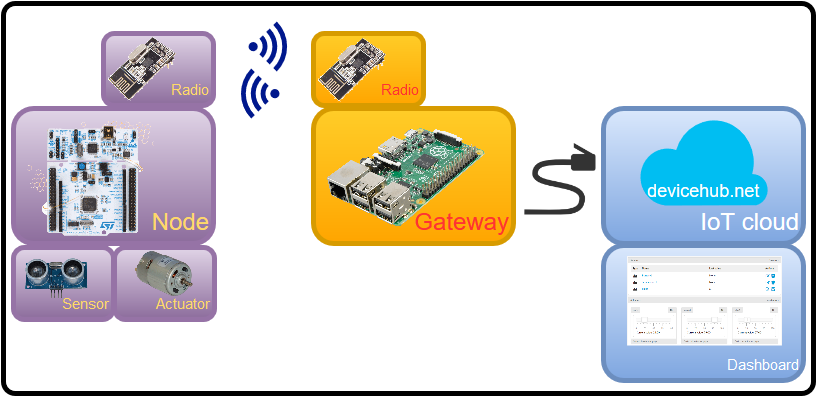
\includegraphics[width=0.9\textwidth]{figures/devices-arrangement.png}
    \caption{Arrangement of devices and components used in this lab}
    \label{fig:meas-arrangement}
\end{figure}

During the exercises a lab report has to be created. In this report the students must document the actions carried out,
the code written, the configuration files created etc. The lab report can also contain screen captures. The basic
guideline is to create such a document of which the measurement is easily reproducible.

\section{Getting started with \emph{\textbf{mbed}} environment}

mbed is an IDE (and also an operating system) tailored for IoT applications based on 32 bit ARM micro-controllers.
There
are several commercially available boards out there as a result it allows simple and rapid prototyping. One of its main
advantages compared to other IDEs that it can handle multiple types of micro-controllers so that the code written can
be reused in multiple environments. Furthermore it has an intuitive UI and also supports on-line workflows with team
integration and version control. Naturally there are some cons as well namely that from mbed the low-level hardware
components are not reachable and sometimes the basis of the framework called \emph{mbed OS} might contain bugs.

The micro-controller used during this lab is of type NUCLEO-F446RE.

\subsection{First steps}

Before proceeding any further do register on site \url{https://developer.mbed.org/}. The registration is simple and
easy
and doesn't require instant verification the e-mail address given. After successful registration log-in on the website
and then
\begin{enumerate}
    \item Go to ``Platforms" tab where the development board is selected
    \item Filter the results for manufacturer of "STMicroelectronics"
\end{enumerate}
\begin{figure}[H]
    \centering
    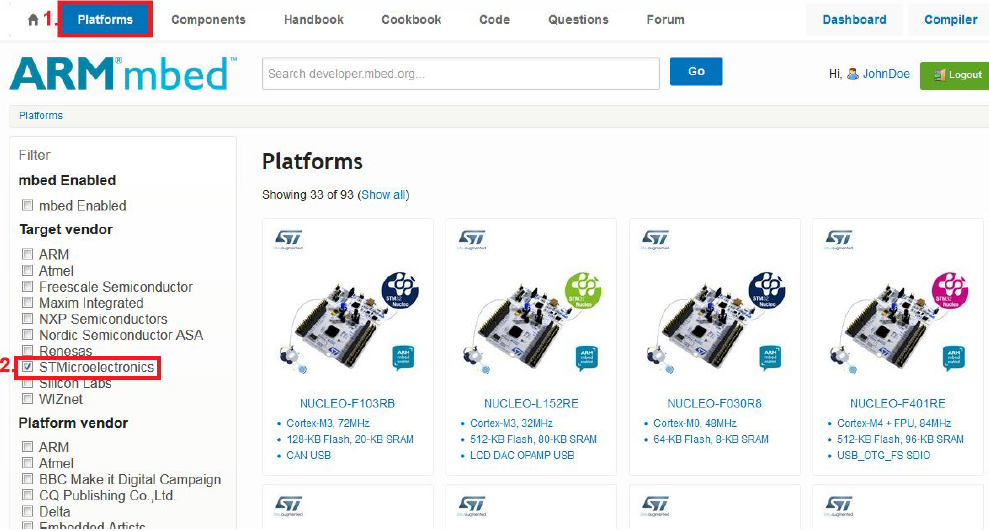
\includegraphics[width=0.9\textwidth]{figures/mbed-platform.png}
\end{figure}
\begin{enumerate}[resume]
    \item Search for and select ``NUCLEO-F446RE" dev board. Here we can find detailed description on the
          micro-controller
          and also the schematics for the pin to feature connector assignment and functions associated with them
\end{enumerate}
\begin{figure}[H]
    \centering
    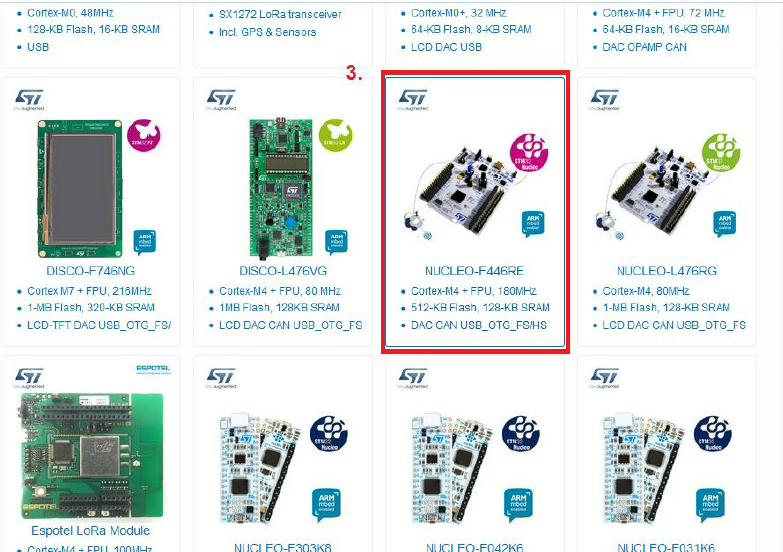
\includegraphics[width=0.9\textwidth]{figures/mbed-nucleo.png}
\end{figure}
\begin{enumerate}[resume]
    \item Add the selected board to the compiler by clicking on the ``Add to your mbed Compiler"
    \item and then open it using the  link in the upper right corner
\end{enumerate}
\begin{figure}[H]
    \centering
    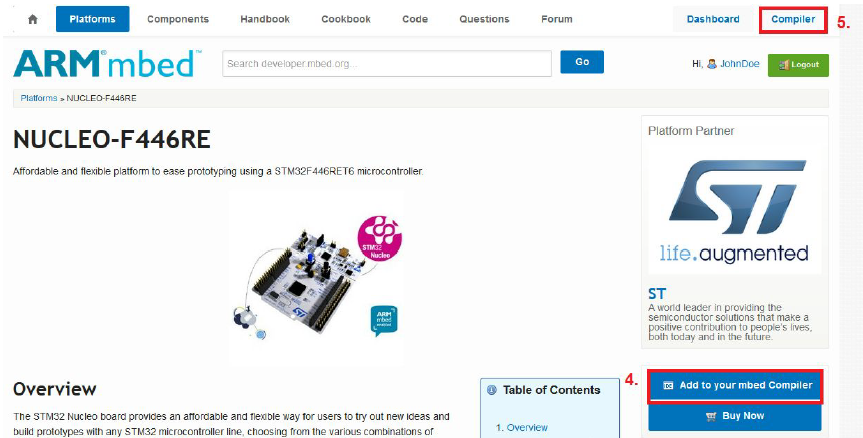
\includegraphics[width=0.9\textwidth]{figures/mbed-compiler.png}
\end{figure}

\subsection{Sample programs and uploading binaries to the device}

Click on ``New" in the top left corner (1.). In the pop-up window (2.) select the appropriate device type, and then
select from one of the existing sample projects (or alternatively create a new one) and provide a name for it. With
the tick-box in the bottom we can select whether to update our code if one of the dependent libraries are updated.
Click on OK and afterwards the newly created program will be visible under the My Programs section under the  provided
name.
\begin{figure}[H]
    \centering
    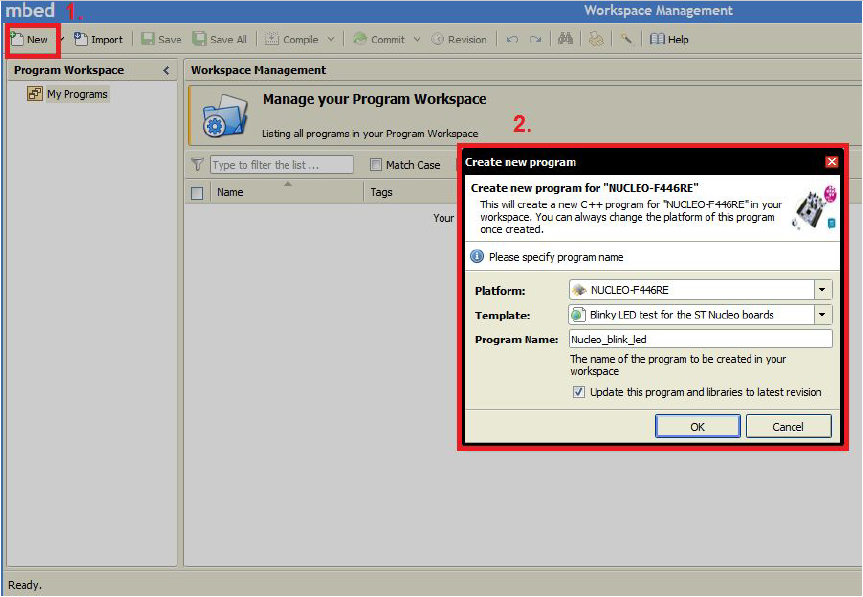
\includegraphics[width=0.9\textwidth]{figures/mbed-new.png}
\end{figure}

We can open and edit (1.) the source files by clicking on it in the left pane. As soon as we are done with the
modifications the compilation can be started by clicking on the ``Compile" button (2.). If there were no errors and the
program compiles successfully the result will be a file download pop-up with the resulting binary (3.)

\begin{figure}[H]
    \centering
    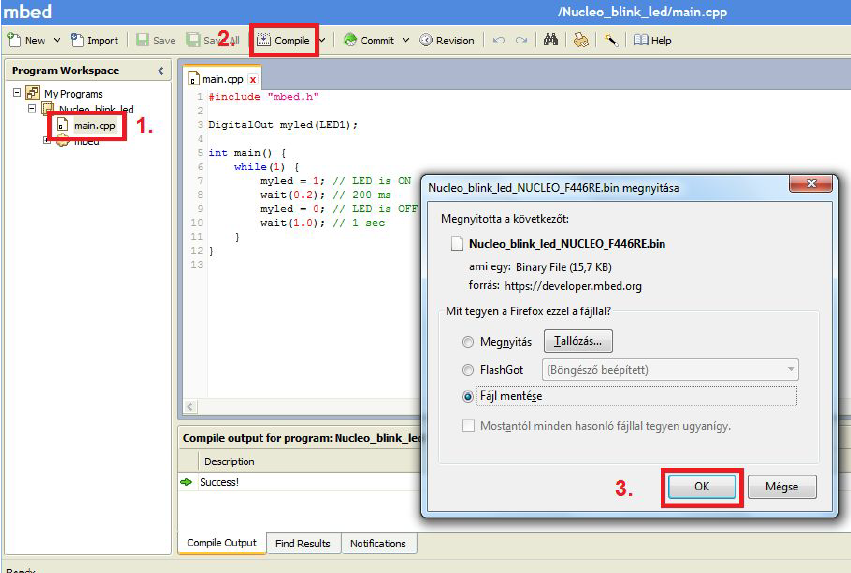
\includegraphics[width=0.9\textwidth]{figures/mbed-compile.png}
\end{figure}

Download/save this binary on the volume created by the dev board (NUCLEO). The green LED will start blinking during
software upload to the micro-controller. If there are no errors our code will start to run on the device immediately.

\begin{figure}[H]
    \centering
    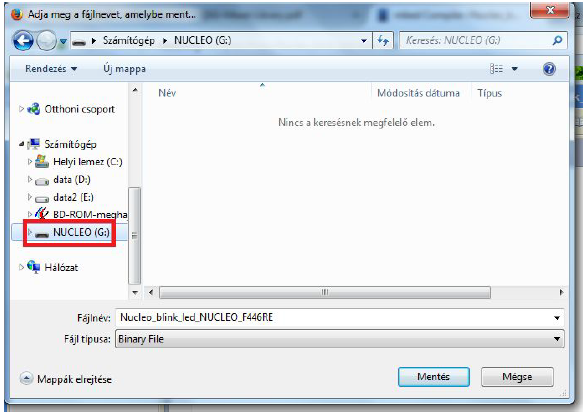
\includegraphics[width=0.9\textwidth]{figures/mbed-nucleo-save.png}
\end{figure}

\subsection{Creating an empty project}
Similarly to the previous steps click on ``New" (1.) then select "Empty Program" option (2.). Name the project (3.)
then click OK. (4.)

\begin{figure}[H]
    \centering
    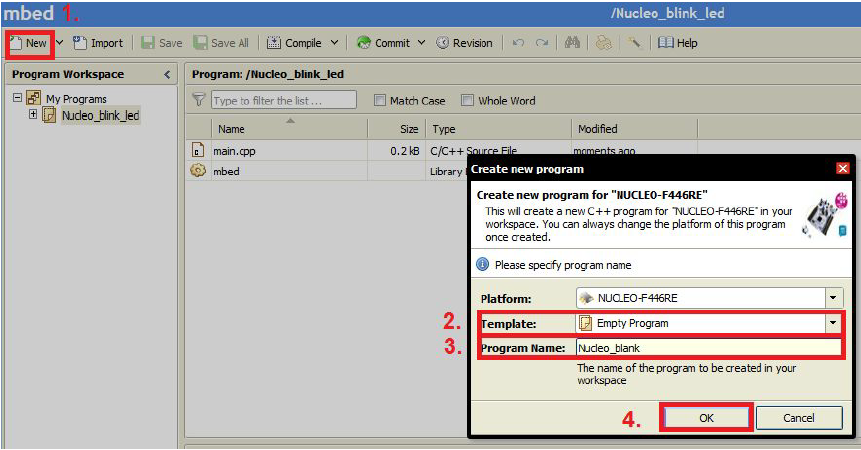
\includegraphics[width=0.9\textwidth]{figures/mbed-empty-proj.png}
\end{figure}

The empty application project needs at least the mbed runtime library that can be added to the project in the following
way:
\begin{enumerate}
    \setcounter{enumi}{0}
    \item Select the project
    \item click on ``Import"
    \item select the ``Libraries" tab
    \item search for the word ``mbed"
    \item Import
\end{enumerate}

\begin{figure}[H]
    \centering
    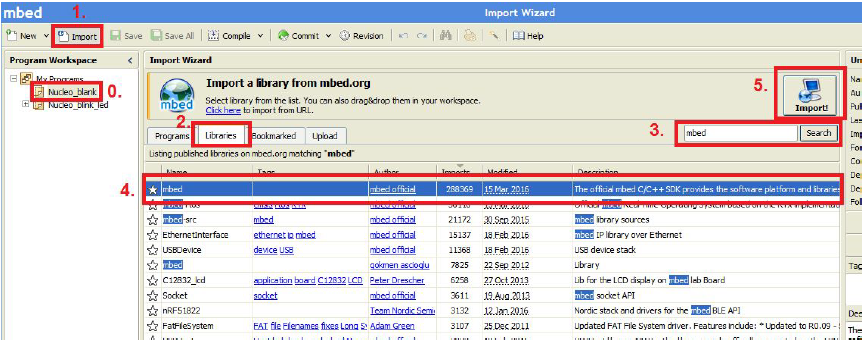
\includegraphics[width=0.9\textwidth]{figures/mbed-import.png}
\end{figure}

\subsection{Different ways of importing}

There are some other ways for importing programs and libraries. A program can be imported based on the above described
method but selecting the ``Programs" tab (1.).
A program or library can be either uploaded from our local machine from a file (2.) or we can download it given that
the url of it is know and we have sufficient privileges.

\begin{figure}[H]
    \centering
    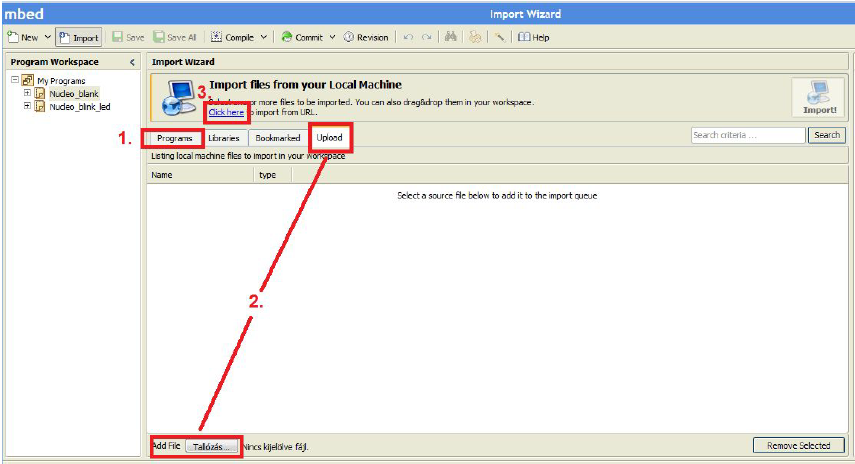
\includegraphics[width=0.9\textwidth]{figures/mbed-import2.png}
\end{figure}

In case if we are a part of a development team there is an option for importing the sources published by other
developers.

\begin{figure}[H]
    \centering
    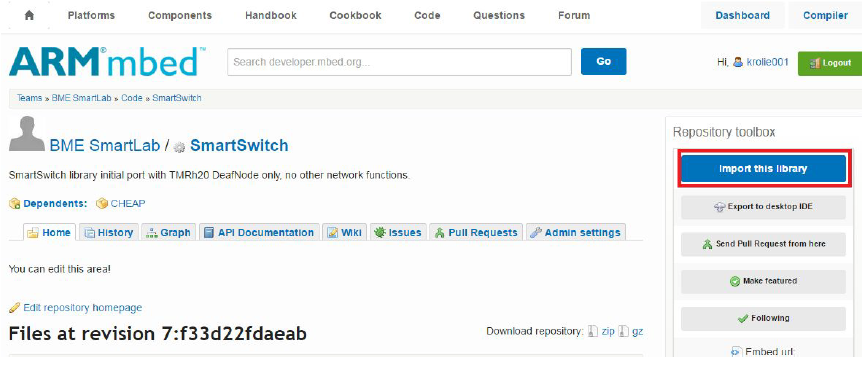
\includegraphics[width=0.9\textwidth]{figures/mbed-online-import.png}
\end{figure}
\begin{figure}[H]
    \centering
    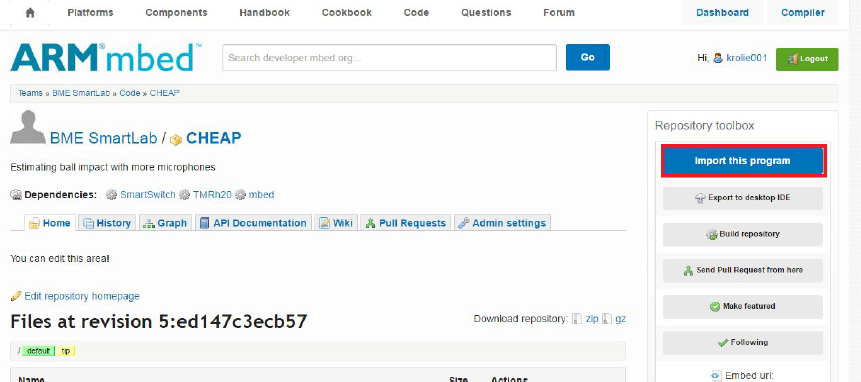
\includegraphics[width=0.9\textwidth]{figures/mbed-online-import2.png}
\end{figure}

\section{Attaching sensors and actuators}

Sensors are available as standalone modules (or simple components). After they are attached to the controller the
sensed data is sent to the micro-controller. The transmission of the data can vary. Simple sensors provide analogue
signals that are digitalized by the micro-controller's A/D converter. More complex sensors digitalize analogue signals
and transmit digital data towards the micro-controller. These devices provide configuration capabilities on top of
reading out data. The communication with these sensors are mainly consists of transmitting command words that are
executed by the sensor and returning the results of the operation for the micro-controller. Complex sensors are capable
of managing other sensors and can return aggregated data for the micro-controller (sensor fusion). The physical
communication standard between a sensor and the micro-controller is usually one of SPI, I2C, USART, OneWire, CAN, etc.
protocols

The sensors used in this lab can be retrieved from the lab demonstrator. A wide variety of sensors are available
ranging from very simple to more complex ones. A complex sensor does not necessary implies a complex attachment
procedure. If one can't find a readily available code for connecting a given sensor it can be written manually during
the class.

\section{Connecting a communication module}

\subsection{Nucleo board pinout}

The Nucleo F446RE board's pinout is shown of Figure~\ref{fig:nucleo-pinout}.

\begin{figure}[H]
    \centering
    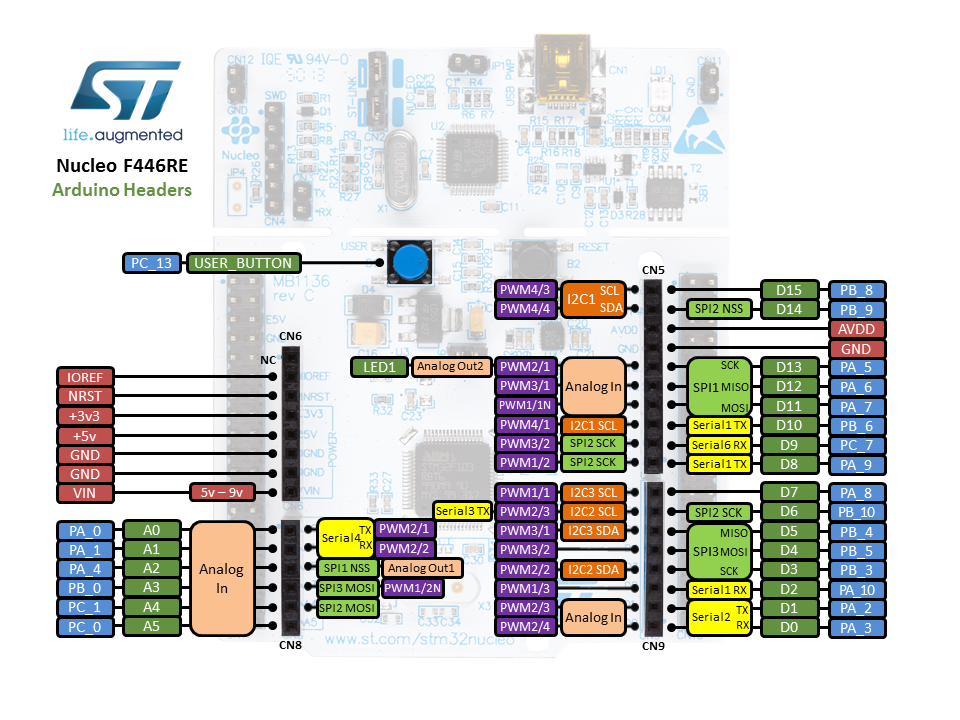
\includegraphics[width=0.9\textwidth]{figures/nucleo-pinout.png}
    \caption{Nucleo F446RE pinout of Arduino headers}
    \label{fig:nucleo-pinout}
\end{figure}

The pins labeled are the female connectors that can be easily addressed from the mbed development environment.
Furthermore all of the 64 male connectors of the Nucleo board are accessible. The male connector headers are found
right
beside the female connector headers the only twist is that on female headers there is a half pin offset due
to providing Arduino compatibility. The neighboring male header does not have this pause that means for a given female
connector it's corresponding male connector is located in the bottom right position from the female pins direction.
Figure~\ref{fig:nucleo-pinout-morpho} illustrates the male connector pinout.

\begin{figure}[H]
    \centering
    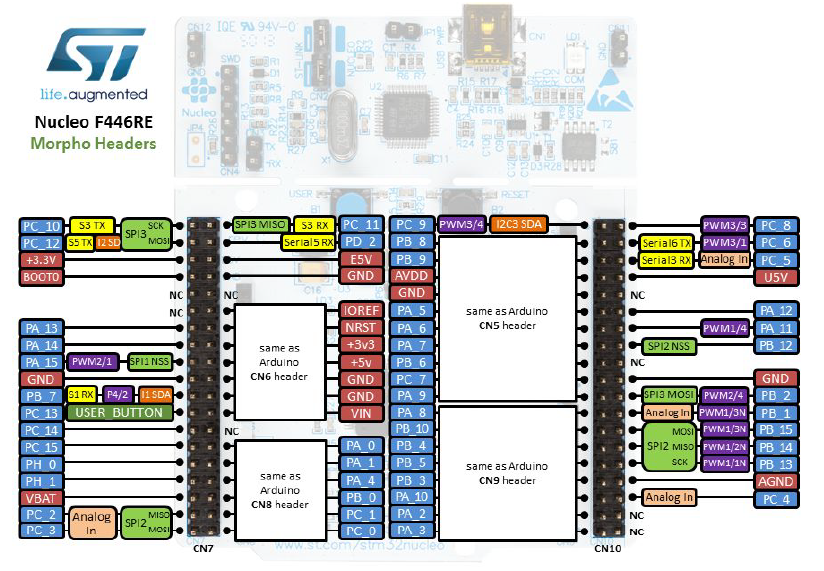
\includegraphics[width=0.9\textwidth]{figures/nucleo-morpho-pinout.png}
    \caption{Nucleo F446RE morpho pinout}
    \label{fig:nucleo-pinout-morpho}
\end{figure}

When supplying power for external devices extreme caution must be taken about the components that require 3.3V power
supply \textbf{MUST NOT} be connected to a 5V supply. (e.g. the radio module requires 3.3V supply).
3.3V power supply is available in three locations: on the Arduino headers there is one male and one female connector
and also on the outer header the 3rd pin from the top on the left side (according to the image).

\subsection{NRF24L01+ module pinout}

The NRF24L01+ radio module is a device communicating on SPI bus. It's important that the power supply must not exceed
3.3V!
In case of improper connection the device will be damaged permanently.
This module has power supply pins (GND,VCC) and SPI bus pins (MISO,MOSI,SCK) and 2 SPI bus control pins (CE,CSN).
Furthermore there is an interrupt pin (IRQ) that is not used in these exercises so that it can be left unconnected.
The pinout of the NRF24L01+ module's pinout is show on Figure~\ref{fig:radio-pinout}

\begin{figure}[H]
    \centering
    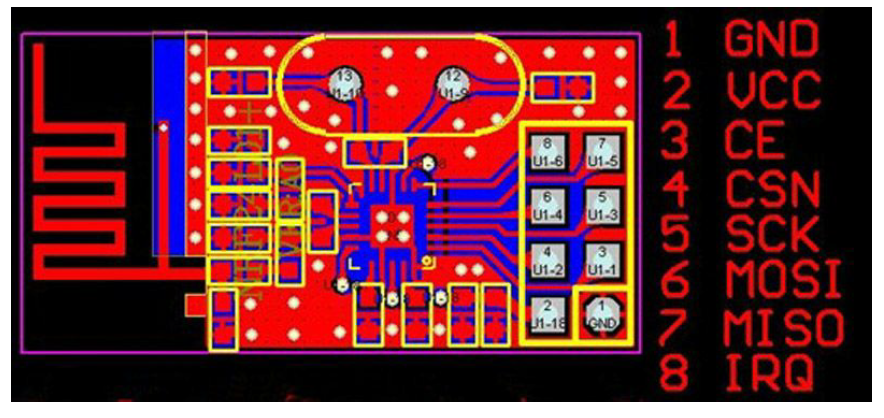
\includegraphics[width=0.9\textwidth]{figures/radio-pinout.png}
    \caption{NRF24L01+ pinout}
    \label{fig:radio-pinout}
\end{figure}

\subsection{Connecting Nucleo and NRF24L01+ modules}

Based on the pinout diagrams connecting the two devices is trivial. There is only one complication about CE and CSN
pins because they can be placed freely. It is advised that D9 and D10 pins are used for this purpose because in that
case they will be collocated with the SPI pins. It must not be forgotten that the radio software has to be adjusted
according to the actual pinout used (NodeConfig class). An example of the interconnection is shown on
Figure~\ref{fig:radio-nucleo-connection}
A sample program for the radio module connection can be downloaded from
\url{https://www.tmit.bme.hu/sites/default/files/attachments/nRF24Test_TMRh20_zip_nucleo_f446re.zip}.

\begin{figure}[H]
    \centering
    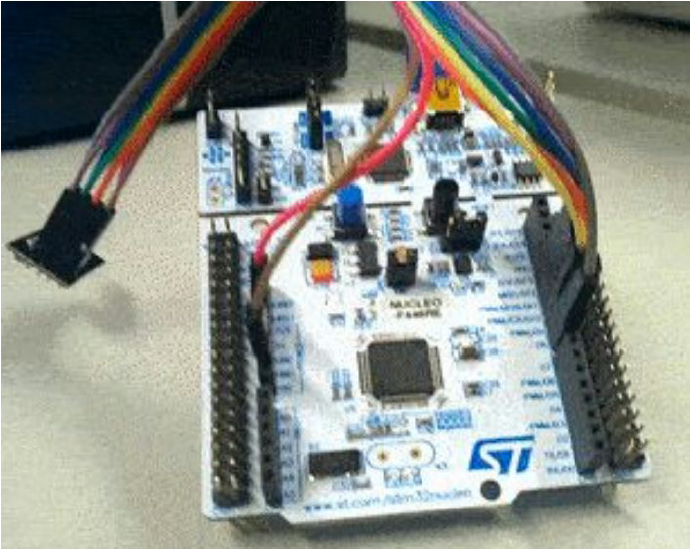
\includegraphics[width=0.9\textwidth]{figures/board-radio-example.png}
    \caption{An example of interconnecting Nucleo F446RE and NRF24L01+}
    \label{fig:radio-nucleo-connection}
\end{figure}

\section{Creating a \emph{virtual device} and communicating with it through DeviceHub.net}

There are multiple service providers offering storage space for IoT applications. It is not only possible to store the
data but also to analyze it. The data upload is realized using the Internet services for which the providers offer an
API. The most popular upload and access mechanism is based on the HTTP protocol but \emph{MQTT} protocol is also
utilized. For this measurement an MQTT based one is going to be used. MQTT is a publish/subscribe based protocol where
the data is sent over appropriate channels (topic) and symmetrically if we want to access some data we need to
subscribe on the desired channel.

\subsection{Creating a project}

As an initial step register on \url{https://dashboard.devicehub.net/register} site then after verifying our e-mail
address log in to the site.
After that in the ``Projects" menu(1.) add a new project (2.):

\begin{figure}[H]
    \centering
    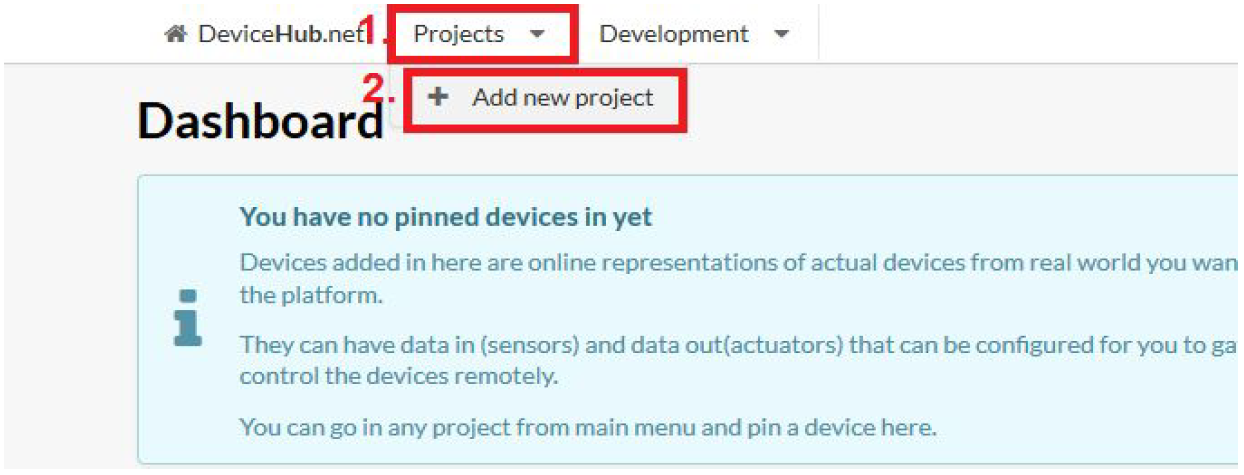
\includegraphics[width=0.9\textwidth]{figures/devicehub-addproject.png}
\end{figure}

In the pop-up window provide an arbitrarily chosen name and click on new project. Optionally an image and description
can be provided for the project.

\begin{figure}[H]
    \centering
    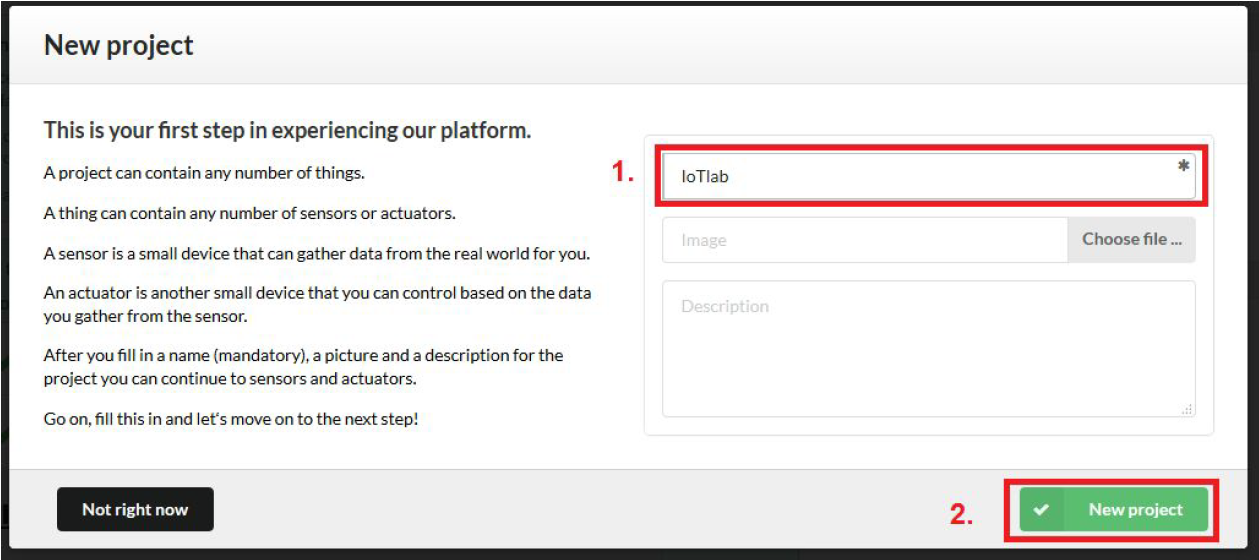
\includegraphics[width=0.9\textwidth]{figures/devicehub-newproject.png}
\end{figure}

On the next page we can add our device and get the unique IDs for the project that are going to be needed later on.

\begin{figure}[H]
    \centering
    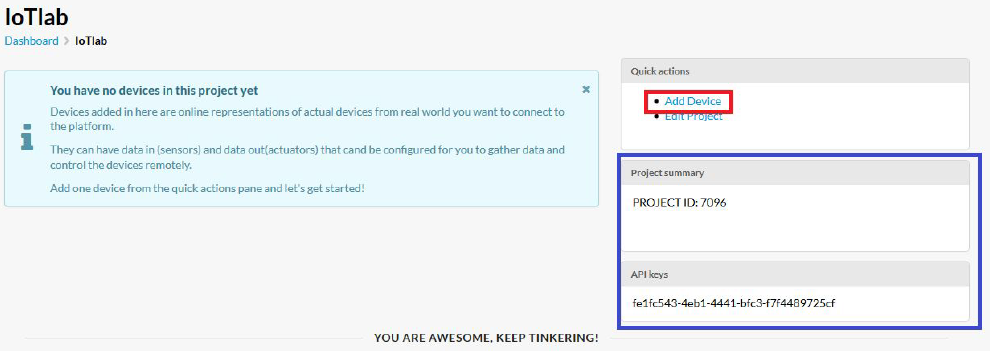
\includegraphics[width=0.9\textwidth]{figures/devicehub-adddevice.png}
\end{figure}

In the pop-up window provide a name for our device. On this same page we can add additional attributes like image and
description but these are not mandatory.

\begin{figure}[H]
    \centering
    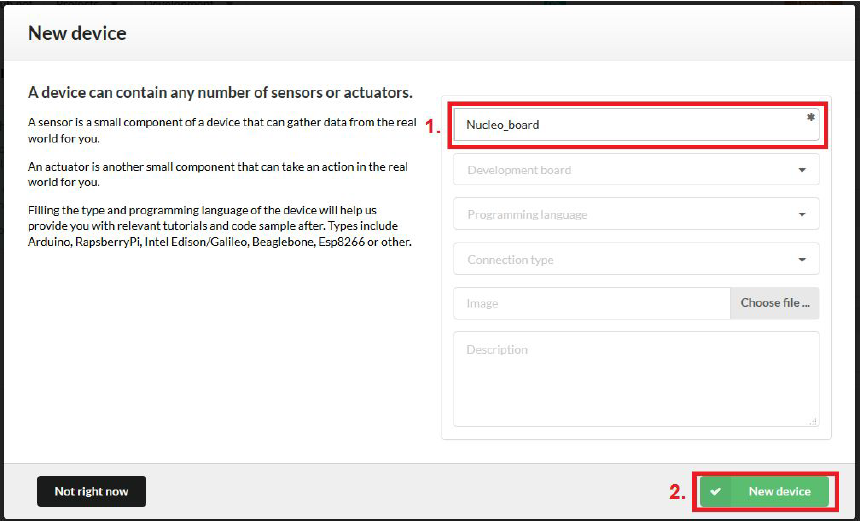
\includegraphics[width=0.9\textwidth]{figures/devicehub-newdevice.png}
\end{figure}

\section{MQTT communication and configuring the Gateway}

The sensor and the actuator communicates within their own networks.
If data transmission over the Internet is required then a \emph{gateway} is required.
The gateway's responsibility is to the place the sensor network data into the appropriate
MQTT channel. Furthermore it also translates/transcodes the data for matching the
data processor's expected format. In this class the sensor network's data is in raw binary format
for providing a compact representation. However the utilized cloud provider expects and sends
data in JSON format. The gateway has to be configured for translating between the two domains.

Code sample for the gateway configuration:
\url{https://developer.mbed.org/teams/BME-SmartLab/code/DeviceHubNet_DEMO/}

\subsection{Introduction to NRF gateway configuration}

In this class the sensor and the actuator communicates with the external world through
a NRF24L01+ radio module. This radio module operates in the ISM band but it is not so
widespread so that its signal can not be received with basic devices and settings. Therefore a
gateway is required that will translate the signals of NRF24L01+ radio module to IP packets
that can be received by any host/program.

The gateway also serves another purpose. Sensors are heavily resource constrained devices as
a consequence the resources used for communication must also be kept at a minimum level.
Therefore the format of the radio communication usually has a compact binary representation.
The maximum frame size of the NRF24L01+ radio is 32 bytes and this also requires a compact transmission
format. In contrast a human readable format is used over the Internet since
the constraints are different over that communication medium and it is more preferred that way.
A commonly used format for describing data is JSON. The second task of the gateway will be then
to translate between the raw binary sensor data and the JSON format used by the IoT cloud.

The third responsibility of the gateway is to perform a mapping between the physical and virtual
devices. The physical sensors are addressed by their micro-controller's network address and an
internal type ID that's valid internally inside a micro-controller domain.
In the virtual domain the devices are identified using different identifiers. The gateway
has to perform an address translation so that the physical and virtual sensors can be paired.

\begin{figure}[H]
    \centering
    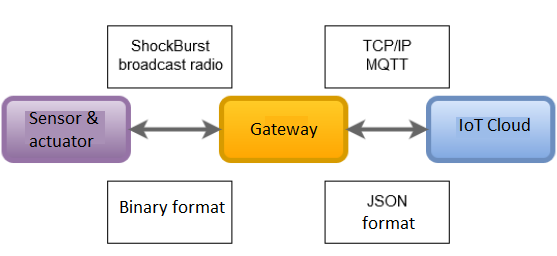
\includegraphics[width=0.9\textwidth]{figures/gateway.png}
    \caption{The end-to-end communication path}
    \label{fig:gateway}
\end{figure}

\subsection{Structure of the Gateway}

The gateway is implemented using a Raspberry Pi micro computer that also has an identical NRF24L01+
radio module just as the sensors. The Internet connection of the gateway is over an Ethernet link.
The Raspberry Pi device is not always located in the lab and it gets its IP address dynamically
that will be specified by the lab demonstrator.

The gateway runs a Debian based Linux distribution. The software components necessary for
implementing the gateway functionality has been pre-installed and will be controlled by the
lab demonstrator. However in order to execute the lab exercises it will be necessary for the students
to log in to the Raspberry Pi and configure their devices. The access details will also be provided
by the lab demonstrator.

\subsection{Radio connection translation}

For radio transmission both the gateway and the sensors use a NRF24L01+ based radio module.
During the measurements the gateway radio operates on a given channel. The sensor's radio
channel has to be aligned with the gateway's radio channel. The current radio channel will be
given by the lab demonstrator.

During the translation the gateway converts the data frames arriving from the NRF24L01+ side
to UDP packets and sends them to a predefined host. As a result of this conversion the
UDP packet will carry the sensor node's network address (2 bytes) and also a microsecond accurate
timestamp (16 bytes) that indicates the time of the frame reception.
Upon receiving an UDP packet the gateway uses the first 2 bytes of the UDP payload as the
network address of the sensor and the remaining part of the payload is sent to the sensor unaltered.
The sensor node will see this as if the gateway with ID 0 has sent a message to it on the radio level, the IP level
source
can not be identified from there.

Another task of the gateway on the radio level is to respond to incoming ``PING" messages.
The sensors are sending ping like messages for testing the radio channel's availability.
The gateway responds with a ``PONG" message for these messages.

\subsection{Content translation}

The translation of the content of the messages is done by a proxy code running on the gateway.
This program is listening on a localhost UDP port and if it receives a packet it runs the
translation logic and sends the results in MQTT format to \emph{devicehub.net}. This program
also subscribes to all MQTT channels on which it expects messages from the direction of \emph{devicehub.net}.
If a message arrives it executes the translation logic then sends the result over the
configured UDP port.

The gateway is configured in way that the previously described radio connection translation
module and the content translator proxy are communicating with each other. This implements a complete
gateway functionality as shown on Figure~\ref{fig:gateway}

\subsection{Message content translation}

The IoT cloud used on this measurement -- \emph{devicehub.net} -- discriminates two types of
data: \emph{ANALOG} and \emph{DIGITAL}. ANALOG type can represent an arbitrary floating point
value while DIGITAL is an on/off type data that can only have values 0 and 1.
During the communication one message can only carry one value as a consequence on the sensor
network side each sensed data element has to be sent in a separate message.

Values of type DIGITAL are translated to 1 byte of payload on the NRF side while the values
of type ANALOG are translated to a 4 byte \emph{float} type. The sensors have to send data
corresponding to these formats.

An example of the translation for the sensor to devicehub direction:

\begin{tabular}{|l|l|l|}
    \hline
                 & Received data                 & Forwarded data                 \\
                 & (payload field, without type) & (data field, without channel)  \\
    \hline
    DIGITAL type & 0x01                          & {"value" : 1}                  \\
    \hline
    ANALOG type  & 0x42 0x2a 0x00 0x00           & {"value" : 42.5}               \\
    \hline
\end{tabular}

An example of the translation for the devicehub to actuator direction:

\begin{tabular}{|l|l|l|}
    \hline
                 & Received data                 & Forwarded data                 \\
                 & (data field, without channel) & (payload field, without type)  \\
    \hline
    DIGITAL type & {"value" : 0}                 & 0x00                           \\
    \hline
    ANALOG type  & {"value" : 33.33}             & 0x42 0x05 0x51 0xec            \\
    \hline
\end{tabular}

For these measurements it is enough to know the translation of these values. In more complex
systems however there are aggregate types or multiple joint data is transferred in one message
(e.g RGB values of a LED) where the translation logic applied is more complex.

\subsection{Address translation}

On the sensor network side -- the NRF24L01+ radio network -- all devices have a network address.
In the original protocol this address is 5 bytes long of which 2 bytes are used now. This is
the unique address of the node. If more than one node has identical unique node addresses
then both will receive the messages however collisions will occur in case of acknowledgments.
The gateway's address is 0.

Inside a node multiple sensors and actuators can be attached to the micro-controller. Typically
of one type there is only one entity so in this demo system the intra node addressing is performed by using
the device type as address. All of the sensors and actuators get a 2 byte type id which is unique only
inside a node. These IDs can be reused in other nodes.

The virtual sensors and actuators have a ProjectID and a DeviceID and also they have a
unique name.

The gateway's responsibility is to translate between physical and virtual identifiers
based on a predefined mapping.

Beside the IDs an API key is required for accessing the virtual devices. This does not
participate in identification however it is necessary to have in order to use the devicehub.net
cloud. This key is also added by the gateway during the translation.

\begin{figure}[H]
    \centering
    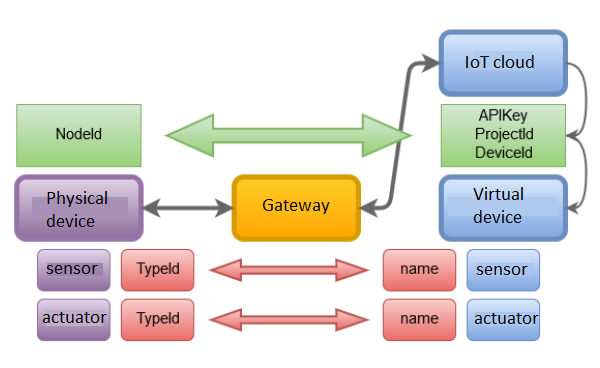
\includegraphics[width=0.9\textwidth]{figures/gateway-addresstranslation.png}
    \caption{The address translation path}
    \label{fig:gateway-addrtransl}
\end{figure}

\subsection{Configuration}

For the radio format translation there is no need for setting any specific configuration.
However it is crucial that the radio parameters must match on the node and gateway side.
The node side settings will be given by the lab demonstrator.

For the message and address translation a configuration has to be prepared for each node
and each sensor and actuator within. The configuration is implemented using a configuration
file. If that is placed to the appropriate place the configuration will take effect immediately.

The name of the configuration file is created from the node's 4 digit id in hexadecimal format.
The file \textbf{node\_1234.json} corresponds to the configuration of node with ID 0x1234. The
task of the students is to create this file for their assigned devices.

A sample config:
\begin{verbatim}
{
    "nodeId": "1234",
    "deviceId": "2533aa65-ff45-aa32-7168-0293e1e5c812",
    "APIKey": "b7beb838-99ee-1278-9845-348414830de2",
    "projectId": "901",
    "things":[
        {
            "sensor": "Light",
            "typeId": 16448,
            "type": "ANALOG"
        },
        {
            "actuator": "LightSwitch",
            "typeId": 16449,
            "type": "DIGITAL"
        }
    ]
}
\end{verbatim}

The \emph{nodeId} field identifies the physical node. The following lines contain the virtual
device identifiers: \emph{deviceId} and \emph{projectId} and the \emph{APIKey} required for
accessing devicehub.net.

The \emph{things} array holds the listing of the mapping of physical and virtual sensors and
actuators. The \emph{sensor} and \emph{actuator} fields are set to values determined by the
virtual device names. The \emph{typeId} field is the one that is used for identifying the
physical sensors and actuators within a node. The \emph{type} field's value is either \emph{DIGITAL}
or \emph{ANALOG} depending on the type of the data.

The prepared configuration file has to be placed under \emph{/home/pi/devicehubproxy/config}
directory on the gateway. After copying the file to the destination directory the configuration
takes place immediately and testing can commence. If there is a need to modify parameters this
file can be updated and the modifications will be in effect immediately.
To create and place this file it is required to log in to the gateway host. The parameters necessary
for logging in to the gateway will be provided by the lab demonstrator. It is also possible
to create and edit the config file while while logged in to the gateway.

Before placing/uploading the file to the destination directory it is strongly advised to check
the JSON syntax for validity. An on-line JSON validator is available on
\url{https://jsonformatter.curiousconcept.com/}.
In case of correct syntax but incorrect operation the lab demonstrator can help in the troubleshooting.

\appendix

\section{Resources}
\begin{itemize}
    \item \href{https://www.tmit.bme.hu/sites/default/files/attachments/IoT1-main.zip}{IoT1-main.zip}
    \item \href{https://www.tmit.bme.hu/sites/default/files/attachments/DeviceHubNet_DEMO.zip}{DeviceHubNet\_DEMO.zip}
    \item \href{https://www.tmit.bme.hu/sites/default/files/attachments/DeviceHubNet_lib.zip}{DeviceHubNet\_lib.zip}
    \item \href{https://www.tmit.bme.hu/sites/default/files/attachments/TMRh20_lib.zip}{TMRh20\_lib.zip}
\end{itemize}

\section{Lab exercises}

\begin{enumerate}
    \item \begin{enumerate}
              \item Hello World
                    \begin{itemize}
                        \item Login to mbed site. Select NUCLEO-F446RE from the available platforms.
                        \item Create a program that blinks the LED on the development board.
                        \item Use the sample codes provided by mbed
                        \item Create a program that controls the LED by the push button found on the board
                        \item Create a program that is able to communicate with the attached PC. Use a serial
                              terminal for the communication.(it's advised to use ``minicom")
                    \end{itemize}
          \end{enumerate}
    \item \begin{enumerate}
              \item Attaching a sensor and an actuator
                    \begin{itemize}
                        \item Pick one-one from the available sensors and actuators and find or create code
                              that will display the sensed data on the PC
                        \item Find the corresponding data sheet of the sensor and study it! While attaching
                              the sensor take care to follow the instructions found in the data sheet.
                        \item Attach the sensor directly to the board or using a breadboard. Use other components
                              if necessary
                        \item Create a program that displays data from the sensor in regular intervals in a compact format.
                    \end{itemize}
              \item Attaching radio comms
                    \begin{itemize}
                        \item Attach the radio unit to the board. The radio uses SPI bus. Identify and connect the
                              appropriate pins. Take care about interference between sensor and the radio!
                        \item Obtain the libraries required for the radio module by either downloading it from the
                              mbed library or from the lab demonstrator.
                        \item Study the radio comms module operation by inspecting the sample code obtained from the
                              lab demonstrator
                        \item Check the operation of the communication at the gateway. Check that the communication is
                              working bidirectionally.
                    \end{itemize}
              \item Bootstrapping the sensor and the actuator
                    \begin{itemize}
                        \item Combine the code of the sensor and the radio communication. Send the data retrieved
                              from the sensor to the gateway.
                        \item Add code created for the actuator to the existing code.
                    \end{itemize}
          \end{enumerate}
    \item \begin{enumerate}
              \item Creating a virtual device
                    \begin{itemize}
                        \item Login to devicehub.net and create a project then create a virtual device.
                              Add the corresponding sensor and actuator to the virtual device.
                        \item Take note of the IDs and data required for accessing the virtual devices
                        \item Examine how can the virtual sensors and actuators be reached using MQTT protocol.
                    \end{itemize}
              \item MQTT communication
                    \begin{itemize}
                        \item Study the MQTT protocol. Examine the components of the protocol.
                        \item Create a connection from an MQTT capable device/software with an MQTT broker then
                              send and receive data using it. The PCs have MQTTfx installed but other software can
                              be used as well.
                        \item Send and receive messages to/from the virtual device. The format and channel of
                              the messages are detailed in the syllabus.
                    \end{itemize}
          \end{enumerate}
    \item \begin{enumerate}
              \item Configuring the gateway
                    \begin{itemize}
                        \item Ask for the access parameters of the gateway from the lab demonstrator.
                        \item Configure the gateway based on the samples provided in order to provided
                              the required translation operation on the appropriate channels.
                        \item Send physical sensor data to the virtual device and also receive virtual data
                              on the actuator.
                    \end{itemize}
          \end{enumerate}
\end{enumerate}

\end{document}